%! Author = chaorn
%! Date = 11.12.24

\section{Das Innere eines Fuzzers}\label{sec:das-innere-eines-fuzzers}
\begin{frame}{Was steckt in einem Fuzzer?}
    \begin{itemize}
        \item \alert{Corpus}
        \item Input Generator
        \item Mutator
        \item Laufzeitumgebung für das zu untersuchende System
        \item Monitoring
        \item \alert{Strategie}
    \end{itemize}
\end{frame}
\begin{frame}{Corpus}
    \begin{itemize}
        \item Sammlung von Testcases (initial händisch)
        \item Wird durch den Fuzzer verwaltet
        \item Wird durch den Mutator verändert
        \item Wird durch den Input Generator erweitert/verkleinert
    \end{itemize}
\end{frame}
\begin{frame}{Input Generator}
    Am Beispiel von AFL(American Fuzzy Lop):
    \begin{itemize}
        \item Generiert Testcases anhand des Corpus
        \item Verwendet bevorzugt Testcases, die zu einer höheren Codeabdeckung führen
    \end{itemize}
\end{frame}
\begin{frame}{Mutator}
    \begin{itemize}
        \item Verändert Testcases
        \item Mutationsstrategien:
              \begin{itemize}
                  \item Bitflips
                  \item Byteflips
                  \item Arithmetische Operationen
                  \item Block Operationen
                  \item Splicing
                  \item \ldots
              \end{itemize}
    \end{itemize}
\end{frame}
\begin{frame}{Laufzeitumgebung}
    \begin{itemize}
        \item Stellt das zu untersuchende System bereit
        \item Am weitesten verbreitet: QEMU
        \item Kann auf verschiedene Arten konfiguriert werden
        \item Sorgt für Isolation des zu untersuchenden Systems
        \item Ermöglicht Cross-Plattform Kompatibilität (z.B.\ Fuzzing von ARM auf x86 Host)
    \end{itemize}
\end{frame}
\begin{frame}{Einschub: Low Level Fundamentals}
    \begin{itemize}
        \item Was ist ein Basic Block?
        \item Was ist Codeabdeckung?
        \item Was ist ein Codepfad?
    \end{itemize}
\end{frame}
\begin{frame}{Low Level Fundamentals}
    \textbf{Basic Block:} Ein Basic Block ist eine Sequenz von Anweisungen, die von einem Punkt im Programmfluss bis zu einem Sprungbefehl führen.\break
    \textbf{Codeabdeckung:} Codeabdeckung ist ein Maß dafür, wie viele Basic Blocks eines Programms durch Testcases erreicht werden.\break
    \textbf{Codepfad:} Ein Codepfad ist eine Sequenz von Basic Blocks, die durch einen Testcase erreicht werden.
\end{frame}
\begin{frame}{Low Level Fundamentals}
    \begin{figure}[H]
        \centering
        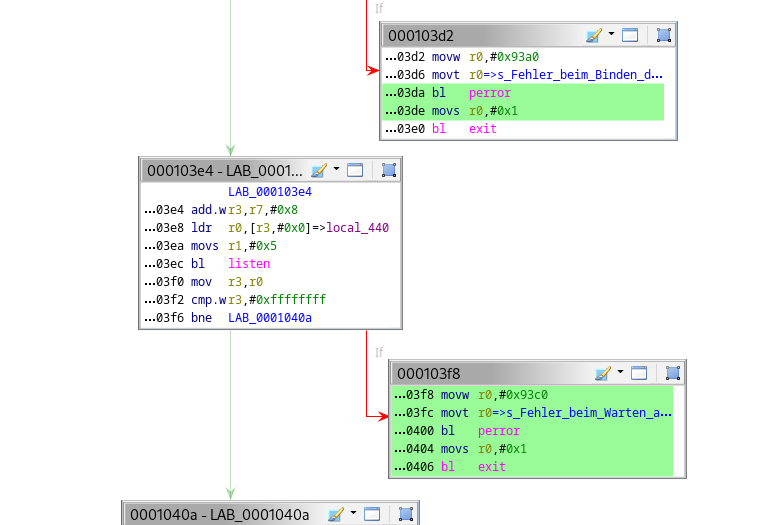
\includegraphics[width=\textwidth]{res/basic_block_example}
        \caption[Basic Blocks am Beispiel eines selbst implementierten TCP Server]{Basic Blocks am Beispiel eines selbst implementierten TCP Server}
        \label{fig:basic-blocks}
    \end{figure}
\end{frame}
\begin{frame}{Low Level Fundamentals}
    \begin{figure}[H]
        \centering
        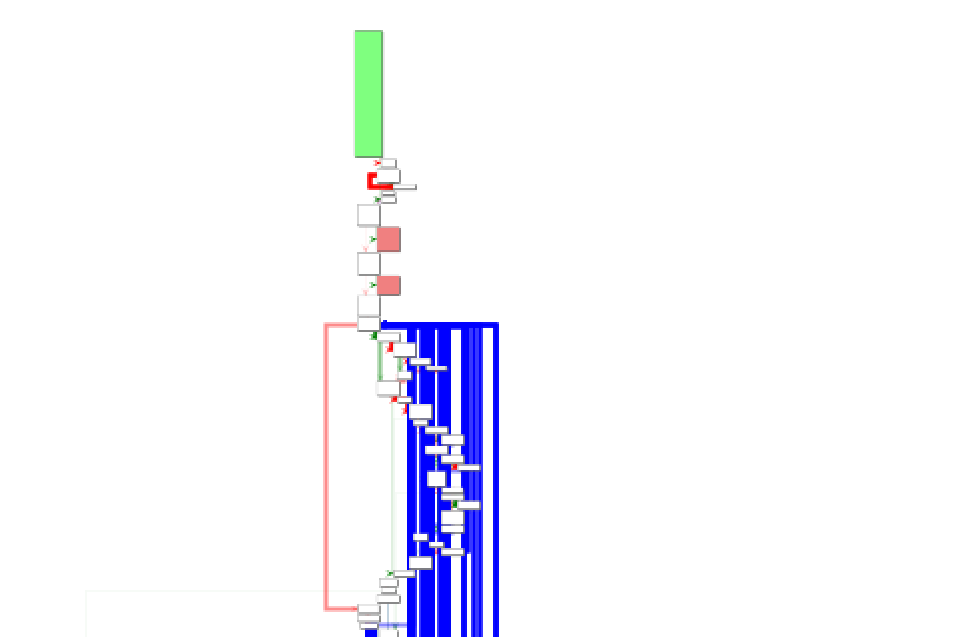
\includegraphics[width=\textwidth]{res/call_graph_ssh}
        \caption[Code Blocks am Beispiel des ssh Binary]{Code Blocks am Beispiel des ssh Binary}
        \label{fig:code-coverage}
    \end{figure}
\end{frame}
\begin{frame}{Monitoring}
    \begin{itemize}
        \item Überwacht das zu untersuchende System
        \begin{itemize}
            \item Codeabdeckung
            \item Laufzeit
            \item Speicherverbrauch
            \item Crashes
            \item \ldots
        \end{itemize}
        \item Oft auf Basis von Instrumentierung
        \item Kann größtenteils über die Laufzeitumgebung realisiert werden
    \end{itemize}
\end{frame}
\begin{frame}{Strategie}
    \begin{itemize}
        \item Steuert den Ablauf des Fuzzers
        \item Bestimmt, welcher Testcase wann verwendet wird
        \begin{itemize}
            \item Codeabdeckung (AFL) = Wie viele (neue) Basic Blocks werden durch den Testcase traversiert?
            \item Zielgerichtet (Dowser) = Spezifische Codepfade, die durch den Testcase erreicht werden sollen
        \end{itemize}
    \end{itemize}
\end{frame}
\section{Techniken des Fuzzings}\label{sec:techniken-des-fuzzings}
\begin{frame}{Techniken des Fuzzings}
    \begin{itemize}
        \item Mutation (AFL)
        \item Generation (boofuzz)
        \item \alert{Machine Learning \& KI} (Pulsar)
    \end{itemize}
\end{frame}
